\documentclass{article}
\usepackage{blindtext}
\usepackage[T1]{fontenc}
\usepackage[utf8]{inputenc}
\usepackage[margin=0.75in]{geometry}
\usepackage{url}
\usepackage{hyperref}
\usepackage{amsfonts}
\usepackage{graphicx}

\begin{document}

\begin{center}

%\LARGE{\textbf{Research Proposal}} \\
%\vspace{1em}
\Large{15-418 Final Project Proposal} \\
\vspace{1em}
\normalsize\textbf{Manish Nagireddy (mnagired) and Ziad Khattab (zkhattab)} \\
\vspace{1em}

\end{center}

\section*{Title}

An Exploration of Parallelism in Neural Networks

\section*{Summary}

For our 15-418 final project, we are looking into potential axes of parallelism that exist within neural networks. We will be implementing neural networks in both C++ (via OpenMP) and Python (via PyTorch and mpi4py, an MPI package for Python) and measuring their performance on CPUs as well as GPUs.

\section*{Background}

In recent years, we have seen the rapid increase of neural networks within the landscape of artificial intelligence, and more broadly within algorithmic decision making. However, because of the large size of these models (given by the number of parameters) as well as the large size of the data used to train them, performance of these so-called deep learning paradigms can be suboptimal without specific attention to parallelism. \\

Broadly, from the perspective of a neural network, there are two dimensions to parallelize: the data and the model.

\begin{enumerate}
  \item \textbf{Data Parallelism:}
  \begin{itemize}
    \item given $X$ machines/cores, split the data into $X$ partitions and use the \textit{same} model to train each partition of the data on a different device in parallel. Then, combine the resultant model weights from each partition
    \item Note that this is model agnostic because it relies only on the data
  \end{itemize}
  \item \textbf{Model Parallelism:}
  \begin{itemize}
    \item splitting the model into various partitions and assigning them to different machines.
    \item NOTE: there are dependencies that are specific to specific model architectures, and so model parallelism is not really ``parallel" because we are actually just assigning consecutive layers of a model to different devices. Some have referred to this as \textit{model serialization}\footnote{\href{https://leimao.github.io/blog/Data-Parallelism-vs-Model-Paralelism/}{Data Parallelism VS Model Parallelism in Distributed Deep Learning Training - Lei Mao's Log Book}}
    \item commonly used when the model is too large to fit on a single device
  \end{itemize}
\end{enumerate}

Refer to the figure\footnote{\href{https://xiandong79.github.io/Intro-Distributed-Deep-Learning}{Link to Figure Citation}} below for an illustration of data parallelism and model parallelism.

\begin{figure}[h]
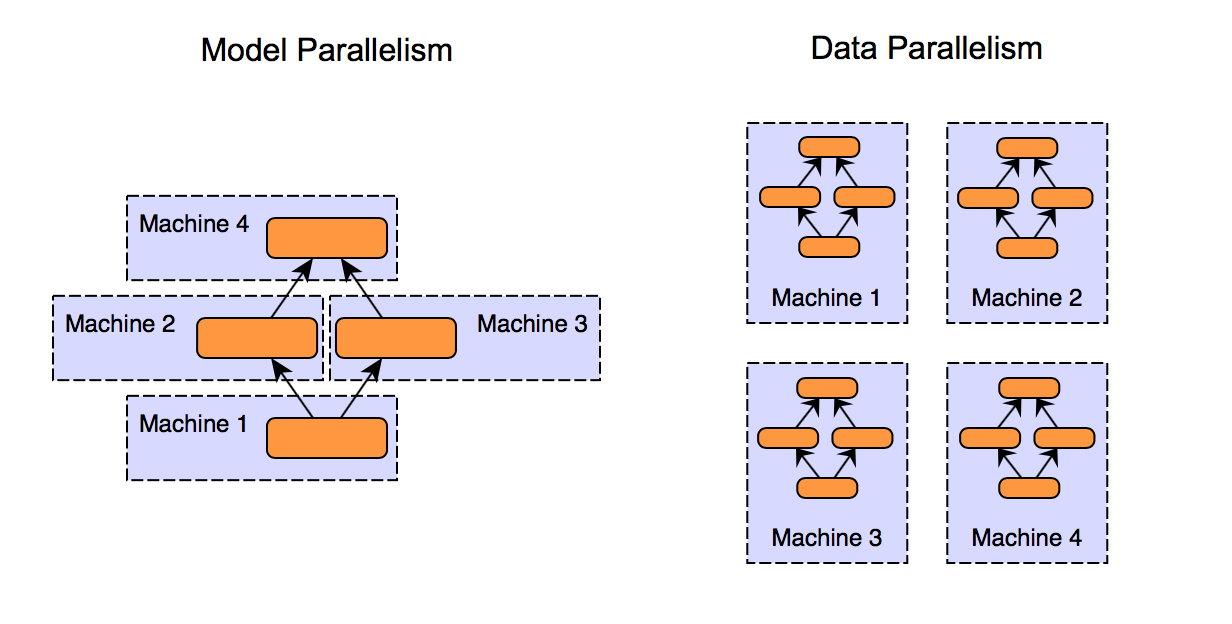
\includegraphics[scale = 0.45]{background}
\centering
\end{figure}

\section*{The Challenge}

\section*{Resources}

\section*{Goals and Deliverables}

\section*{Platform Choice}

\section*{Schedule}

\end{document}
